\section{Szenariokonstruktion}
\label{constructions}
Als dritte und wichtigste Phase der Szenarioanalyse werden nun Szenarien aus den vorher definierten Einflussfaktoren erstellt. Hierfür bietet es sich an, die vorher ermittelten Entwicklunsausprägungen der einzelnen Schlüsselfaktoren auf Widerspruchsfreiheit zu überprüfen . Dafür wird eine Konsistenzanalyse genutzt \cite{spath}. Auf dessen Grundlage werden danach zukunftsfähige Anwendungsszenarien für die Skola GmbH erstellt.

\subsection{Konsistenzanalyse}

In der in Abbildung \ref{fig:konsistenzanalyse} dargestellten Konsistenzanalyse erhält man eine Übersicht über die Beziehung zwischen den einzelnen Ausprägungen. Der Übersichtlichkeit halber wurden die einzelnen Ausprägungen abgekürzt. Die Erklärungen finden sich in Abschnitt \ref{manifestations}.

\begin{figure}
	\centering
	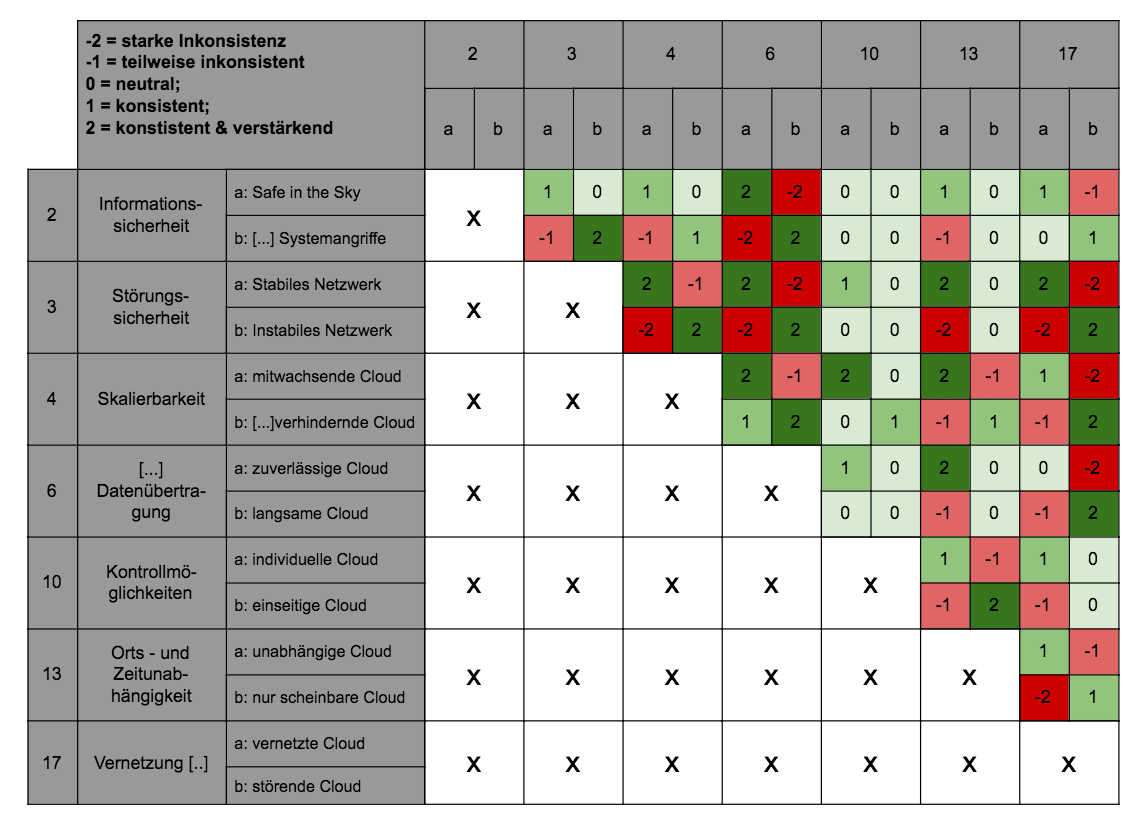
\includegraphics[width=\linewidth]{images/konsistenzanalyse}
	\caption[Caption for parameters]{Konsistenzanalyse}
	\label{fig:konsistenzanalyse}
\end{figure}

Für die Konsistenzanalyse wurde eine Skala zwischen -2 (starke Inkonsistenz) und 2 (konsistent und verstärkend) gewählt. Faktorenausprägungen, die eine starke Inkonsistenz aufweisen, können nicht zusammen in einem Szenario aufgeboten werden \cite{spath}. Andersrum können aus verstärkenden Ausprägungen Cluster gebildet werden, woraus sich Szenarien abbilden lassen.

Aus der Analyse der Schlüsselfaktoren auf Widerspruchsfreiheit lässt sich sehr gut erkennen, dass sich die jeweiligen Best-Case Ausprägungen zumeist verstärken. Besonders lässt sich ein positives Cluster aus den Ausprägungen \textit{Stabiles Netzwerk} (3a), \textit{mitwachsende Cloud} (4a), \textit{zuverlässige Cloud} (6a) und \textit{unabhängige Cloud} zusammenfassen. Andere positive Ausprägungen lassen sich zudem hinzuaddieren, sodass sie weiterhin verstärkend wirken. Im Gegensatz dazu verstärken sich die negativen Ausprägungen der Schlüsselfaktoren, wodurch sich ein entsprechendes negatives Cluster bilden lässt.

Aus dieser Betrachtung lässt sich erschließen, dass sich die Vorteile des Cloud Computing generell verstärkend aufeinander auswirken. Ebenso unterstützen sich die Risiken gegenseitig in ihrer Ausprägung. Diese Erkenntnis kann nun zur Hilfe gezogen zu werden, um drei mögliche Zukunftsszenarien für das Cloud Computing im Bildungsbreich zu erstellen.

\subsection{Szenario 1 - Mobiles Lernen auf dem Vormarsch}

In diesem Zukunftsszenario haben die positiven Ausprägungen des Cloud Computing Einklang in den Lernalltag von Schülerinnen und Schülern gefunden. Mobiles Lernen ist kein Ideal mehr sondern ein allgemeiner Zustand. Lernende haben jederzeit und überall Zugang zu Materialien über das Internet. E-Learning gehört ebenso zum Alltag wie eigenverantwortliches Nacharbeiten zu Hause mit dem eigenen Smartphone oder Tablet. Den Schülerinnen und Schülern wird Platz für freie Entfaltung gegeben, klassischer Unterricht besteht nur noch geringfügig. Schulbücher in der Form wie man sie aus klassischen Lernprinzipien kennt existieren bestenfalls als Zusatzmaterial. Große Schulbuchverlage wie Cornelsen oder Westermann haben ihre Angebote längst ins Internet mithilfe von Cloud Services verlagert. Dadurch bieten sie flexible, aber auch zahlreiche Lernmaterialien für jeden an. Zudem sind die angebotenen Dienstleistungen jederzeit sicher und entsprechen sämtlichen Datenschutzrichtlinien. 

In Betrachtung der derzeitigen Entwicklung des Cloud Computing ist ein solches Szenario in den nächsten 10-15 Jahren denkbar. Der Gebrauch der Technologie wächst immer weiter an \cite{krcmar} und Firmen der deutschen Bildungsindustrie überdenken ihr Angebot hinsichtlich eines Wechsels zu cloudbasierten Diensten \cite{grella}.

\subsection{Szenario 2 - Blended Learning (Hybrid)}

Dieses Szenario sieht ein Mischmodell aus Online - und Offline-Angebot von Unterrichtsmaterialien vor. Dies entspricht der in Abschnitt \ref{futuretrends} vorgegebenen Definition des \textit{Blended Learning}. Es sollen Synergien beider Modelle genutzt werden, um Vorteile beider Seiten auszunutzen und Nachteile möglichst zu beseitigen. Das Szenario sieht vor, dass Schülerinnen und Schüler eigenständig Hausaufgaben oder Nachholarbeiten über das cloudbasierte Web Services vornehmen, zum Beispiel durch E-Learning Angebote. Weiterhin bestehend bleibt aber der eigentliche Präsenzunterricht. Unterstützt wird dieser durch passende Web Services, die den Unterricht didaktisch bereichern \cite{meinel}.

Dieses Szenario ist ebenfalls in den nächsten 10-15 Jahren als ziemlich realistisch einzuschätzen. Zwar bleibt das Vertrauen in bewehrte Unterrichtskonzepte, auch hervorgerufen durch die Angst vor Datenschutzverletzungen, jedoch steigt der Einsatz von Cloud Diensten rasant \cite{krcmar}. 

\subsection{Szenario 3 - Zu hohe Risiken}

Eher unwahrscheinlich ist das dritte Szenario, welches beschreibt, dass Cloud Computing gar keinen Einklang in die Bildungsbranche finden wird. In diesem Fall sind die abgeschätzten Risiken der Technologie zu groß, um ernsthaft Vertrauen in eine Verlagerung von Lernmaterialien in die Cloud zu gewinnen. Hier wird weiter bewährte, klassische Konzepte vertraut. 

Unrealistisch ist dies deshalb, weil die Vorteile des Cloud Computing bei weitem überwiegen. Zwar gibt es berechtigte Risiken, wie zum Beispiel die Datensicherheit oder die Störanfälligkeit der bereitgestellten Infrastrukturen, diese können jedoch durch geeignete Konzepte eingeschränkt werden.

